\section{Feature}
In order to explore the insightful  information of musical head movement, we extract several feature from the original accelerometer data:
\begin{itemize}
\item{\em Wave amplitude},which is the difference of a wave bottom and its next wave peak. It measures the acceleration when the user performs the head movement, in other words, wave amplitude describes “how hard” the user nod his head. Due to accelerometer data usually contains high frequency noise, and we are more interested in the main signal where user nod his head, a 5-Hz-cutofflow-pass filter is applied before we detect peaks and bottoms in the signal .   
\item{\em Wave widh}, which is the time interval between two bottoms or two peaks. It describes the time to complete one nodding movement. The user is stimulated by a music cue, wave width is affected by the time interval between beats.
\item{\em Series of response time (SRT)},which is the series of time interval between the music beat and corresponding movement. Studies in ~\cite{eye blink} and ~\cite{tap beat} show this feature could be used to differentiate the users. Note that user is not necessary responding after the beat, as he can anticipate if he is familiar with the music cue. Thus, response time in our measurement can be either negative or positive. However, finding the associated movement is a non-trivial process, hence we develop the following algorithm for a robust detection. First, accelerometer data needs to be synchronized with the music cue in midi format. Note that midi file is a time series of instrument commands,  no additional signal processing is required to detect the beat in the music as we can take each command as a beat if the music is simple enough. Second, we locate two neighboring peaks where a beat resides in between, and compute the time intervals from the beat to both peaks. Finally, we choose the one with a smaller absolute value as the response time. In some cases,  user is not necessary nodding for every beat,  thus we use the 90 percentile of the response time sample to interpolate  when the detecting response time is beyond this value. 
\end{itemize}
\begin{figure}
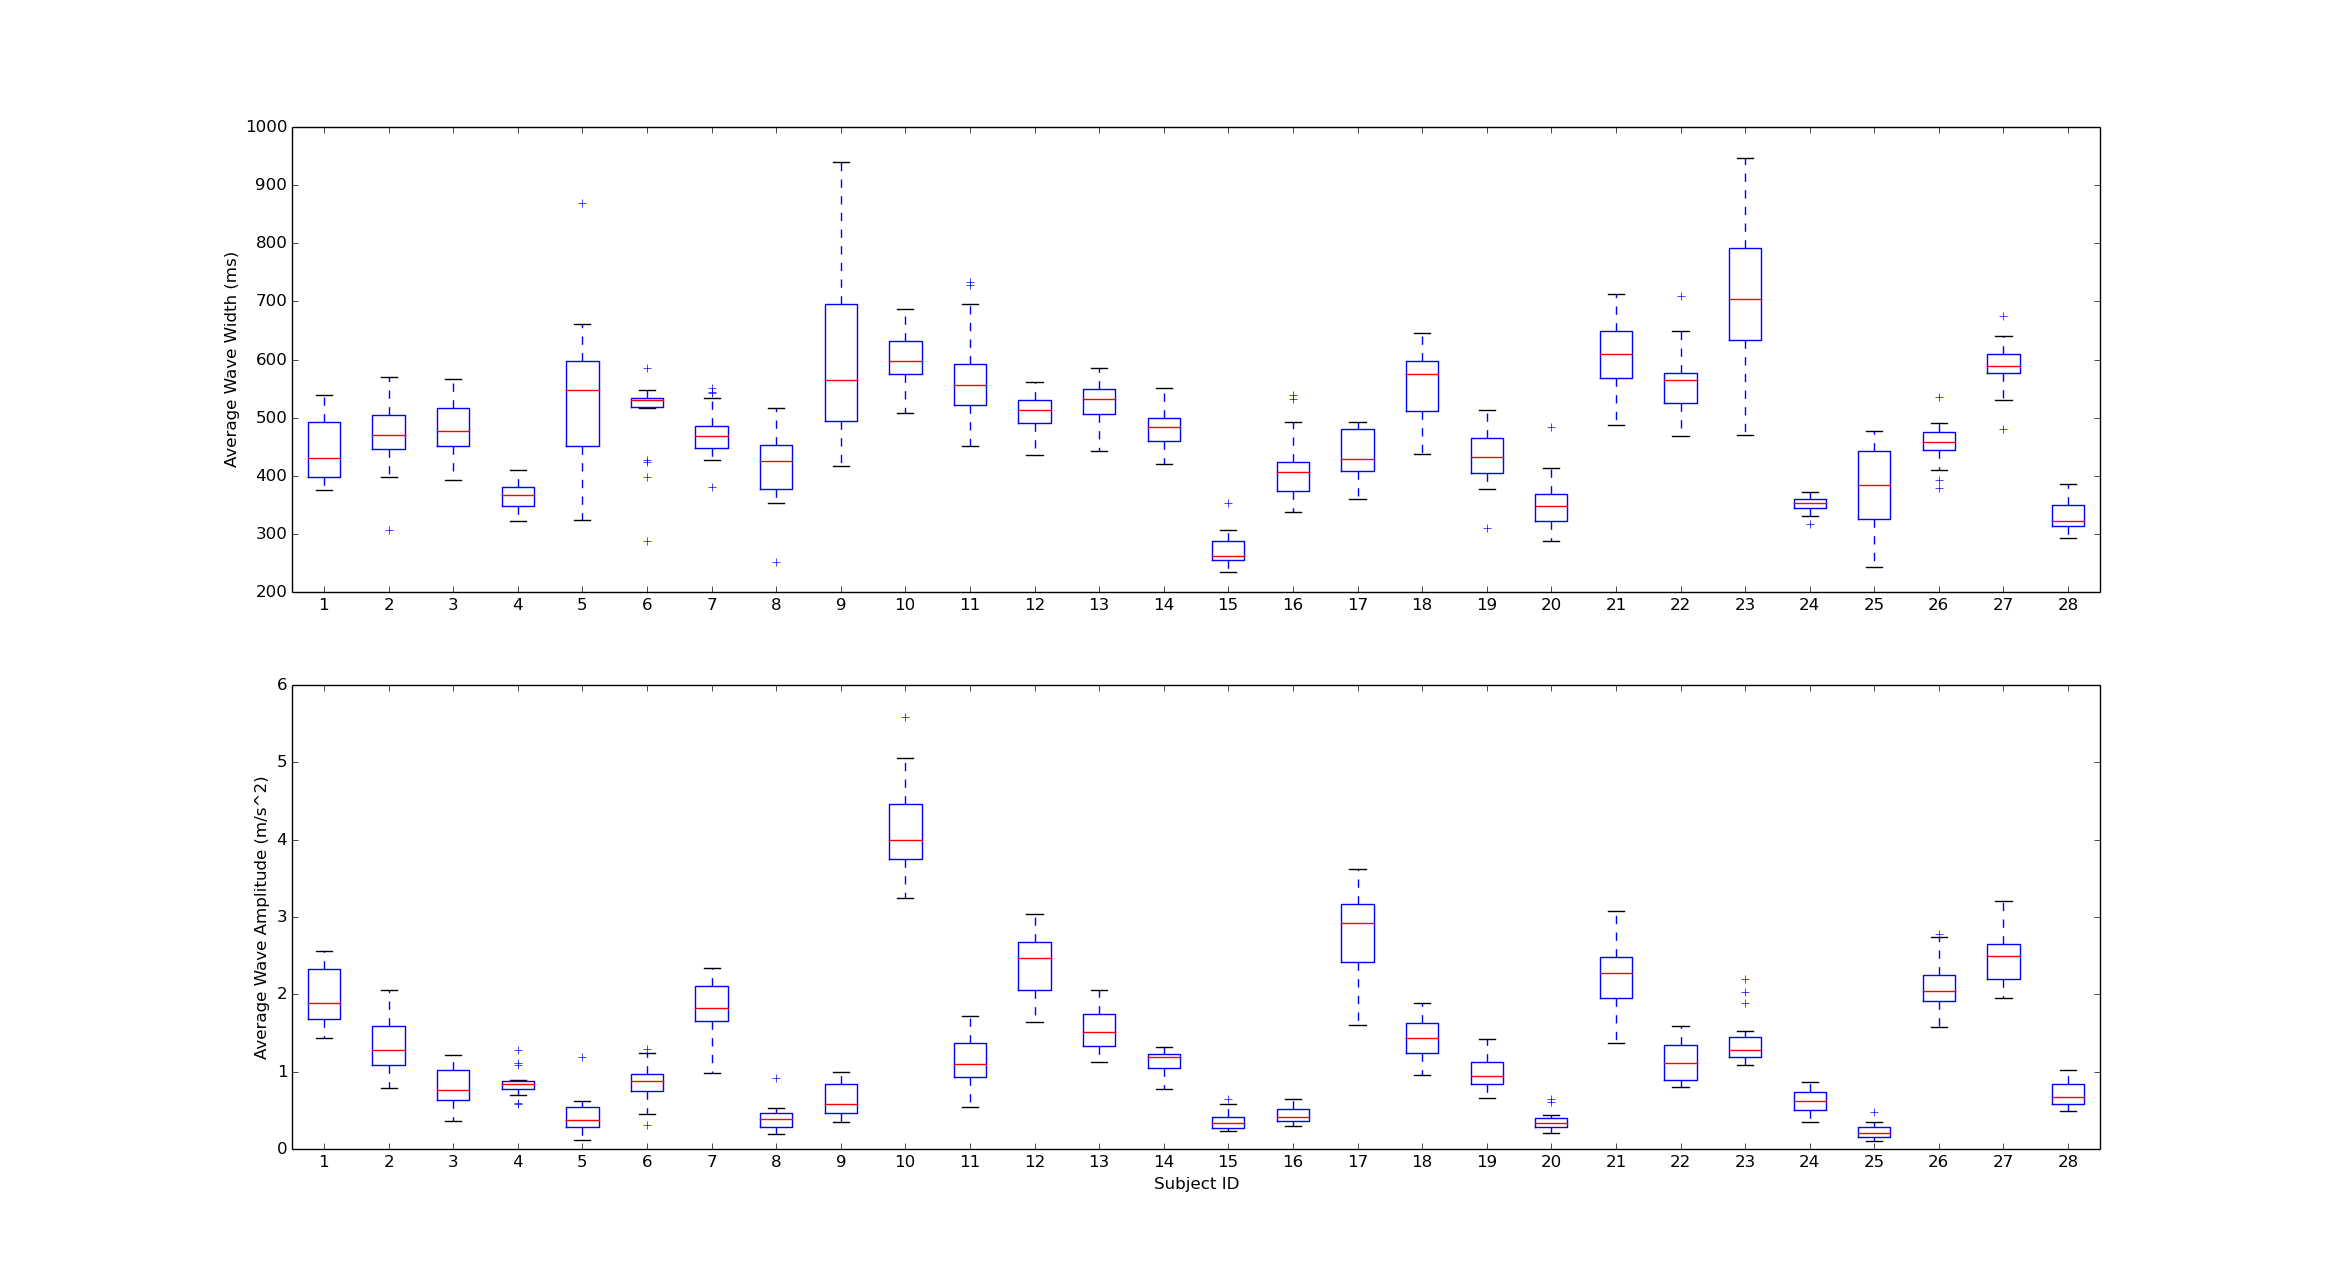
\includegraphics[width=\columnwidth]{figure/width_amp_box.png}
\caption{\label{fig:width_amp} Wave Amplitude and Width Boxplot}
\end{figure}

\begin{figure*}[t]
\begin{center}
\begin{tabular}{ccc}
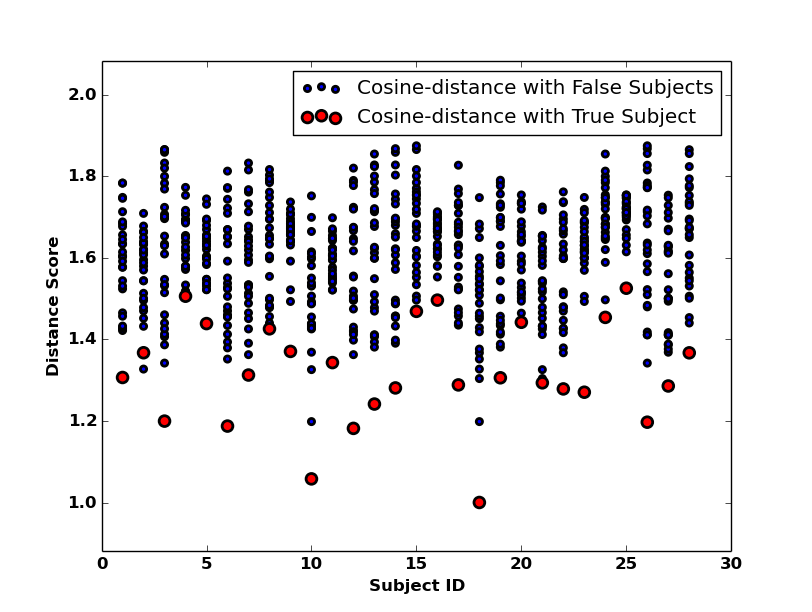
\includegraphics [width=.33\linewidth]{figure/resp_time_cos.png}&
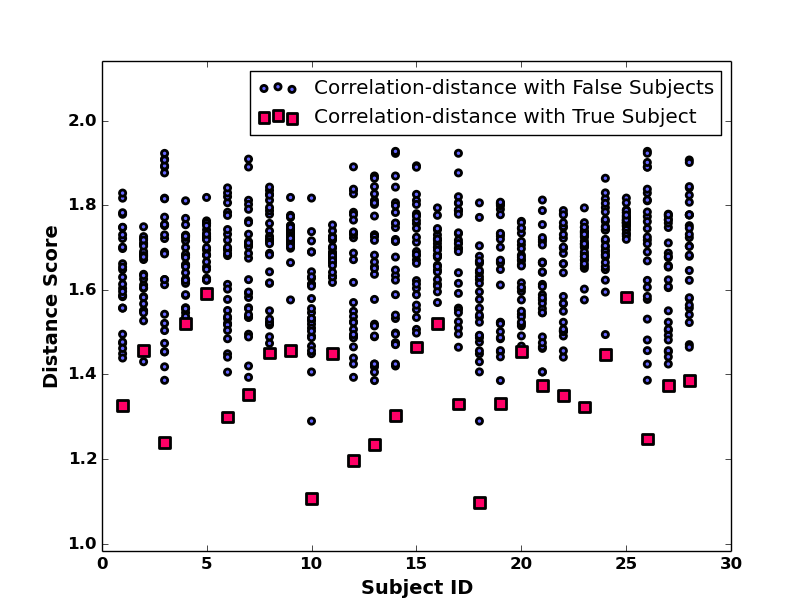
\includegraphics [width=.33\linewidth]{figure/resp_time_cor.png}&
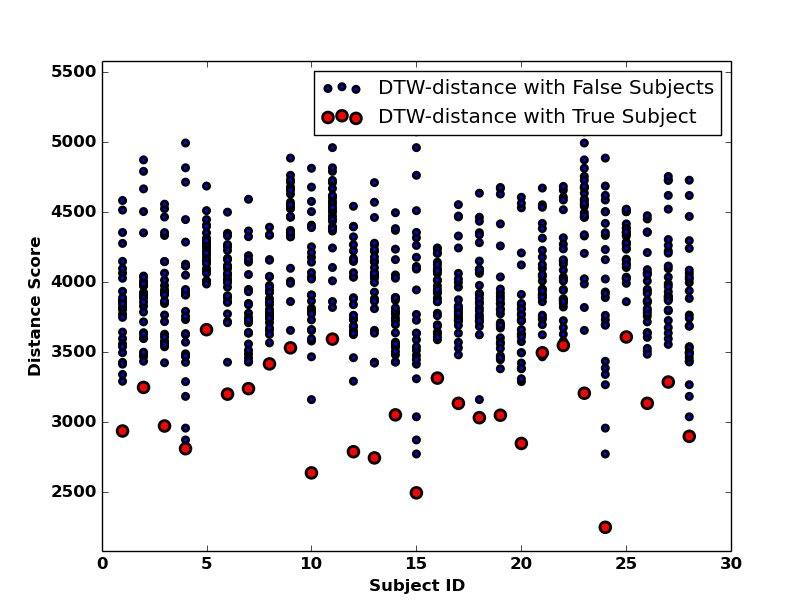
\includegraphics [width=.33\linewidth]{figure/resp_time_dtw.png}\\
(a) Cosine Distance & (b) Correlation & (c) DTW \\
\end{tabular}
\end{center}
\caption{\label{fig:distance} The similarity score is computed over N (N = 20) sample data for each subject, and 28 subjects in total. For each column, a red dot represents the average similarity score of that subject's own SRT, i.e., each of his sample data compared with the other N-1 SRTs from him, hence we have the average similarity score over all these comparison. Similarly, a blue dot on the same column represents the similarity score of that subject's SRTs compares with another subject's SRTs.}
\vspace{-2pt}
\end{figure*}


As shown in Figure~\ref{fig:width_amp}, most subject ’s wave amplitude are with different means and small variance compared with their wave width.  To better understand the SRT for different users,  we apply various similarity scores to provide an intuitive and quantitative description of their difference. In Figure~\ref{fig:distance}, Cosine Distance (COS) and Correlation (COR) can help most of the subject to differentiate himself with the other subjects, but for some subjects's true subject score (red dot) are closed to their false subject score (blue dot). For subject 2, red dot even exceeds the blue dot.The output Dynamic Time Warping (DTW)~\cite{cite dtw} can be used as another distance metric. ***describe why DTW is better than the other two in this case***. In Figure~\ref{fig:resp_time_dtw}s,  it shows that all average self-comparing similarity scores are lower than that when they are compared with others. The observation above indicates the possibility to further derive a system which can differentiate the true user and the false users based on the fusion of these features.